\section{Introduction}
\label{sec:intro}


Temporal sentence grounding in video (TSGV) aims to locate the target video clip corresponding to the query sentence, which plays a vital role in fields such as video creation and video monitoring. 
With the help of deep learning, TSGV has achieved promising performance~\cite{RN2, RN3, RN4, RN5, zheng2023generating, wang2023scene}. 
However, recent studies~\cite{RN7, RN28, RN29} have shown that TSGV models are susceptible to dataset biases. 
They perform the grounding task through shortcuts created by dataset biases rather than the alignment between query texts and corresponding visual regions, resulting in poor generalization performance.

From the perspective of the dataset distribution, 
given samples that contain similar semantic components in the input video or query text, the bias originates from the uneven temporal distribution of the corresponding target moments. 
As shown in Figure~\ref{Introduction}, in the widely used ActivityNet dataset, for samples containing the word ``see'' in the query text, their target moments tend to be concentrated in the first half of the video, and only a few target moments are located elsewhere in the video. This uneven distribution leads to unexpected spurious correlations between query words and target moments, which are easily captured by TSGV models. Once the query contains the word ``see'', the model will predict the target moment as the first half of the video with a high probability. 
Similar phenomena also exist in the visual modality. 
Hence, generating samples to break these correlations and form a uniform temporal distribution of target moments is an effective debiasing strategy. 


\begin{figure}[t]
	\centering
	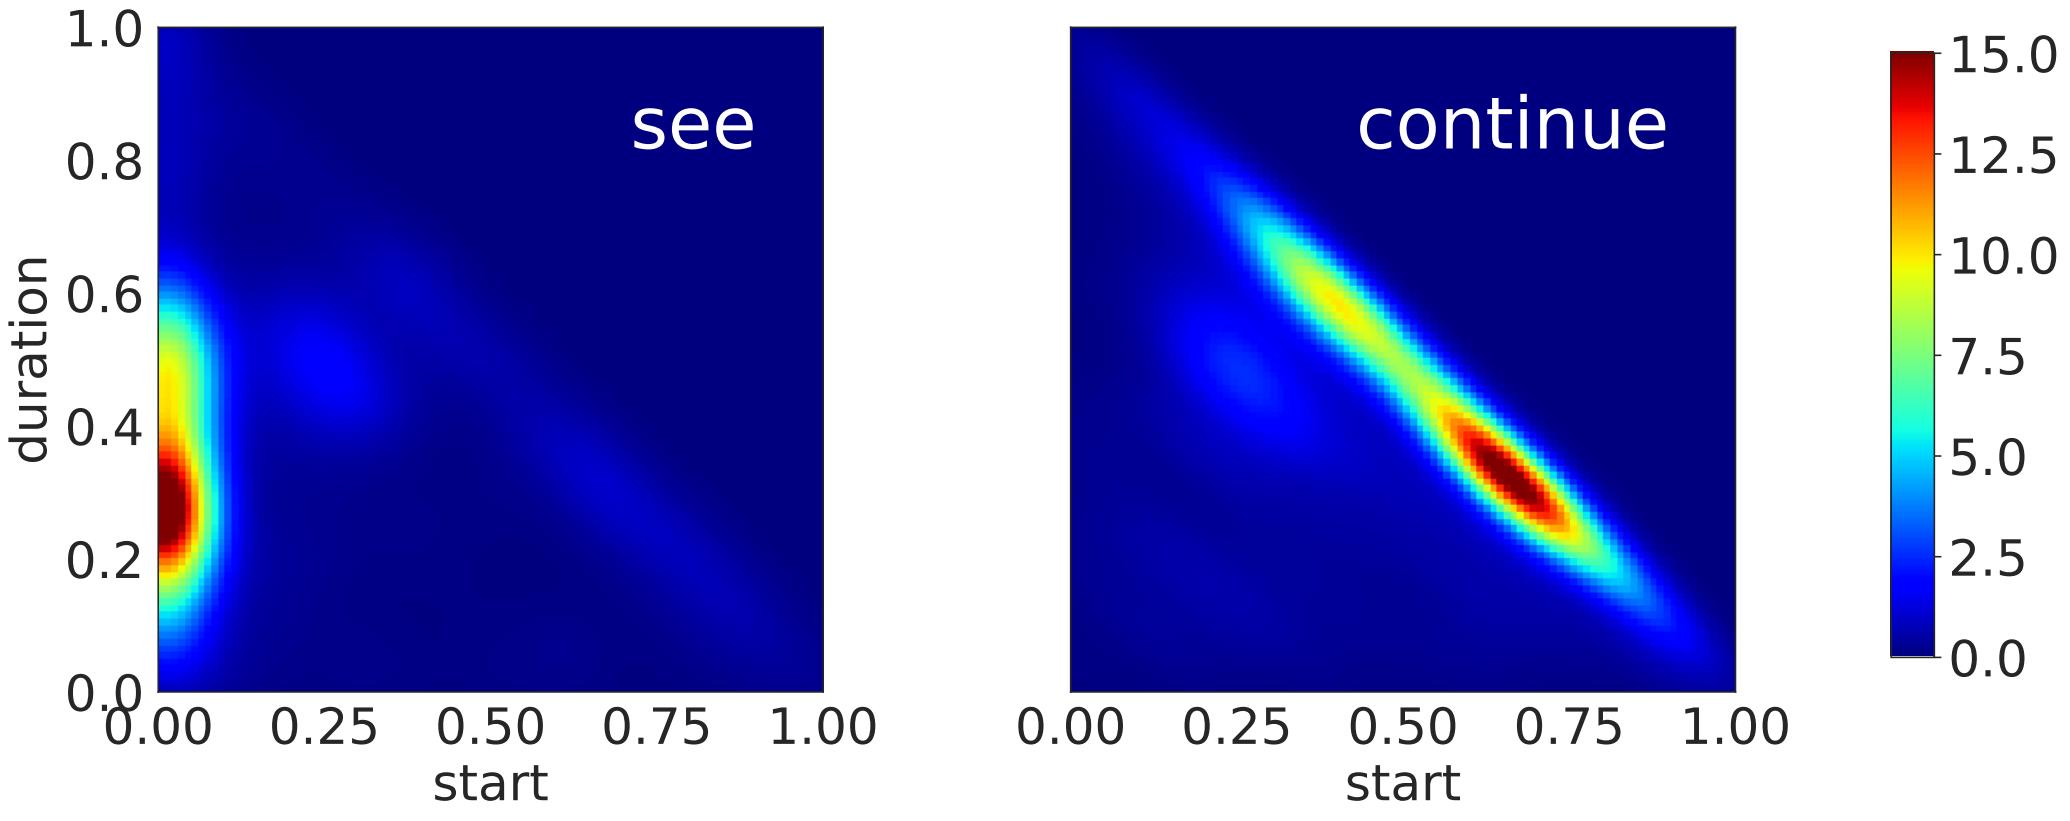
\includegraphics[width=\linewidth]{images/Introduction.jpg}%.pdf}
	\caption{The spurious correlation between query words and temporal location of target moments. The horizontal and vertical axes represent the normalized starting time and duration of the target moment, respectively. The color represents the text-video pair density, which is obtained by using kernel density estimation with the Gaussian kernel.}
	\label{Introduction}
\end{figure}


However, due to the rich semantic content in the video and text, we can not enumerate all the coupling relationships between the target moment and the semantic component of the video/text to generate corresponding samples. It is impossible to construct an ideal dataset without dataset biases. 
Therefore, Zhang {\it et al.}~\cite{RN31} modify the relative positions of target moments through video clipping to form a more uniform temporal distribution of target moments. 
Liu {\it et al.}~\cite{RN28} replace certain verbs or nouns in the query with similar vocabulary from the dataset to obtain negative samples for the coupling relationship between query words and target moments. 
These methods only disrupt a fixed quantity of dataset biases because of the limited diversity of words in the dataset and the limited relative positions of target moments. 
%Besides, they can not break the coupling relationship between visual features and target moments.

Based on the above analysis, we propose the bias-conflict sample synthesis and adversarial removal debias strategy (BSSARD) for TSGV. 
Its core idea is that in the training stage, we randomly generate fake target moments for each real sample. Then we use the bias generator to generate visual or linguistic bias features condition on these fake target moments and construct bias-conflict samples that are falsely associated with the synthetic target moments. Through adversarial training, the bias discriminator should accurately judge that the bias-conflict sample contains biases and predict the original target moment. 
In essence, it will generate some samples for all the spurious correlations between the temporal position of the target moments and the visual/text modality data. 
It greatly destroys the uneven temporal distribution of the target moments in the TSGV datasets and disrupts language and visual biases simultaneously. 
%Besides, our method can adaptively generate corresponding bias-conflict samples according to the dynamic change of the bias relationships that the main model relies on in different training stages.

Specifically, BSSARD consists of two bias generators and a grounding model with a bias discriminator. Given a video-text pair $(I_v,I_q)$ with target moment $(y_s^r, y_e^r)$, BSSARD will iteratively generate visual/text bias-conflict samples to form real and fake samples for adversarial debiasing. We first randomly generate a fake target moment $(y^f_s, y^f_e)$. 
Mimicking the spurious correlation between the visual feature and the fake target moment, we use the visual bias generator to produce a bias vector based on $(y^f_s, y^f_e)$, and add it to the visual feature of $I_v$, which constructs the bias-conflict sample $(\tilde{I_v},I_q)$. Through $(\tilde{I_v},I_q)$, the visual bias generator aims to force the grounding model to produce $(y^f_s, y^f_e)$ and determine the input is a sample without bias. 
Instead, the grounding model needs to produce $(y_s^r, y_e^r)$ for $(I_v,I_q)$ and determine it is a sample without bias. Meanwhile, it should also produce $(y_s^r, y_e^r)$ for $(\tilde{I_v},I_q)$ and determine it is a sample with bias. 
For the query bias generator, the process is similar. 
Through adversarial training, bias generators continuously introduce biases and generate bias-conflicting samples to deceive the grounding model.
Meanwhile, the grounding model continuously eliminates the introduced biases, which requires it to model cross-modality alignment information to accomplish the grounding task. 
Hence, the final model can effectively resist the influence of dataset biases and achieve better generalization performance.

Experimental results on the repartitioned Charades-CD and ActivityNet-CD datasets demonstrate the effective debiasing capability of our approach. 

Our main contributions are as follows: 
\begin{itemize}
	\item We propose a novel debiasing strategy, which generates bias-adversarial samples for most dataset biases and performs debias through adversarial training. 
	\item We propose a debias network with two bias generators, a grounding block, and a bias discriminator, which can effectively eliminate visual and language biases. 
	\item Extensive experiments on the OOD-test set demonstrate that BSSARD achieves great debias performance.
\end{itemize}
